\documentclass{article}
\usepackage{graphicx} % Images
\usepackage{amsmath,amsthm} % Math
\usepackage{wasysym,MnSymbol} % Greek alphabets
\usepackage{mathrsfs,amsfonts,calrsfs} % Math fonts
\usepackage{newtxtext}
\usepackage{geometry} % Formatting
\usepackage[dvipsnames,svgnames]{xcolor}
\usepackage[strict]{changepage}
\usepackage{framed}
\usepackage{cancel}
\usepackage{autobreak}
\usepackage{hyperref}

\graphicspath{ {./images/} }

\providecommand{\tightlist}{
  \setlength{\itemsep}{0pt}
  \setlength{\parskip}{0pt}}

\newcommand*\sepline{%
  \begin{center}
    \rule[1ex]{.5\textwidth}{.5pt}
  \end{center}}


\setlength{\parindent}{0pt}% cancel indentation before every line

% right cases
\newenvironment{rcases}
  {\left.\begin{aligned}}
  {\end{aligned}\right\rbrace}

% Blue block
\definecolor{blueshade}{rgb}{0.95,0.95,1} % blue block color
\newenvironment{blueblock}{
\def\FrameCommand{
  \hspace{1pt}
    {\color{DarkBlue}
    \vrule width 2pt}
    {\color{blueshade}
    \vrule width 4pt}
  \colorbox{blueshade}
}
\MakeFramed{
  \advance
  \hsize-
  \width
  \FrameRestore}
\noindent\hspace{-4.55pt}% disable indenting first paragraph
\begin{adjustwidth}{}{7pt}
\vspace{2pt}\vspace{2pt}
}
{\vspace{2pt}\end{adjustwidth}\endMakeFramed}


% Green block
\definecolor{greenshade}{rgb}{0.90,0.99,0.91} % green block
\newenvironment{greenblock}{%
\def\FrameCommand{%
  \hspace{1pt}%
    {\color{Green}%
    \vrule width 2pt}%
    {\color{greenshade}%
    \vrule width 4pt}%
  \colorbox{greenshade}%
}%
\MakeFramed{%
  \advance%
  \hsize-%
  \width%
  \FrameRestore}%
\noindent\hspace{-4.55pt}% disable indenting first paragraph
\begin{adjustwidth}{}{7pt}%
\vspace{2pt}\vspace{2pt}%
}
{%
\vspace{2pt}\end{adjustwidth}\endMakeFramed%
}


% Red block
\definecolor{redshade}{rgb}{1.00,0.90,0.90} % red block
\newenvironment{redblock}{
\def\FrameCommand{
  \hspace{1pt}
    {\color{LightCoral}
    \vrule width 2pt}
    {\color{redshade}
    \vrule width 4pt}
  \colorbox{redshade}
}
\MakeFramed{
  \advance
  \hsize-
  \width
  \FrameRestore}
\noindent\hspace{-4.55pt}% disable indenting first paragraph
\begin{adjustwidth}{}{7pt}
\vspace{2pt}\vspace{2pt}
}
{\vspace{2pt}\end{adjustwidth}\endMakeFramed}


\newtheorem{question}{Question}
\newtheorem{note}{Note}
\newtheorem{proposition}{Proposition}
\newtheorem{lemma}{Lemma}
\newtheorem{property}{Property}


\title{Notes on Advanced Macroeconomics}
\author{Victor Li}
\date{Spring Sememster, 2024}

\begin{document}

\begin{titlepage}
   \vspace*{\stretch{1.0}}
   \begin{center}
      \Large\textbf{Notes on Advanced Microeconomics}\\
      \large\textit{Victor Li}\\
      \large\textit{Autumn semester, 2023}
   \end{center}
   \vspace*{\stretch{2.0}}
\end{titlepage}

\newpage
\tableofcontents

\newpage
\addcontentsline{toc}{section}{Preface}
\section*{Preface}

Aim of this work of mine is to provide clear macroeconomic knowledges in language as simple as possible. Most of this note is taken from the advanced macroeconomics course of Yanfei Deng I took. This note is still a work in progress and needs tons of ammending. See the newest version at \url{https://github.com/xolarvill/notes-on-economics} along with my other notes. And pull a request if you figure some part of this note is wrong.

This work was first written in markdown language on Obsidian, which provides a lightweight and highly personalized working experience. But it was later transfered into purely latex language on Sublime Text, due to poor support for rendering of long math equation blocks of Obsidian. For the tranfer I used Pandoc at \url{https://pandoc.org/}. I wrote some LaTeX snippets of Sublime Text to optimize the writing experience, and uploaded on github at \url{https://github.com/xolarvill/snippets-for-quick-latex-on-st}.

One can find enormous academical help on advanced macroeconomics from books listed below:
\begin{itemize}
\tightlist
  \item Introduction to Modern Economic Growth, D. Acemoglu
  \item Economic Growth, R. Barro and S.i.M. Xavi
  \item The ABCs of RBCs, An Introduction to Dynamic Macroeconomic Models, G. McCandless
  \item Macroeconomics, A Comprehensive Textbook for First-Year Ph.D. Courses in Macroeconomics. M. Azzimonti, P. Krusell, A. McKay, and T. Mukoyama
  \item Adavanced Macroeconomics, D. Romer
\end{itemize}


\newpage
\part{Consumer and demand theory}

\newpage
\section{Choice set}
A single choice or a single consuming plan is denotes as
$$x=(x_{1},x_{2}...x_{n})\in \mathbb{R}_{+}^{n}$$

A choice set or a consuming set is a set of possible and mutually exclusive alternative consuming plans, denoted as 
$$X= \mathbb{R}_{+}^{n} $$
It represents all plans of consuming goods, regardless of possibility.

A choice set should at least fulfil the following requirements:

1. choice set is not a null set
$$\phi\neq X \subseteq \mathbb{R}_{+}^{n}$$

2. $X$ is closed, in this way, also continuent.

3. $X$ is convex, denoted as
$$\forall x^{1},x^{2}\in X, \forall \lambda\in[0,1],\lambda x^{1}+(1-\lambda)x^{2}\in X$$

4. $X$ can contain zero, meaning the choice maker can choose to not consume.
$$0\in X$$

\section{Preference relationship}
\textbf{Preference relationship} is a binary relationship defined on $X$:
in the choice set $X$, $\forall x,y,z \in X$, preference relationship (at least as good as) is denoted as
$$x\succsim y$$

\begin{blueblock}
\begin{note}
Preference relationship $\succsim$ is defined on $X$, so its minimum unit is a consuming plan $x=(x_{1},x_{2},...,x_{n})$.
e.g.: $x_{1}\succsim x_{2}:(x^{1}=1,x^{2}=3)\succsim (x^{1}=5,x^{2}=1)$
\end{note}
\end{blueblock}

\textbf{Restrict preference relationship} is denoted as 
$$x\succ y \iff x \succsim y, \; y \neg\succsim x$$

\textbf{Indifference preference relationship} is denoted as
$$x \sim y \iff x \succsim y, y\succsim x$$

\textbf{Rational preference}

Given a relationship $\succsim$ in a non-empty choice set $X$, we call $\succsim$ a rational preference if it possesses three properties(axioms):
\begin{align}
&1.(transitivity) \; x\succsim y,y\succsim z \Rightarrow x\succsim z
\\&2.(completeness) \; x\succsim y \lor y\succsim x
\\&3.(reflectivity) \;\forall x\in X, x\succsim x
\end{align}

\begin{blueblock}
\begin{note}
Many pyschological experiments ended up with results overthrowing the transitivity axiom. But for now, we assume it to hold true.
\end{note}
\end{blueblock}


Some propositions: if the $\succsim$ is rational:

\begin{proposition}[i]
\text{$\succ$ is not reflective($x\succ x$ does not hold true) but transitive($x \succ y,y\succ z \Rightarrow x\succ z$). This means $\succ$ is not rational.}
\end{proposition}

\begin{proof}
\begin{align}
&Let \;\exists x \in X, x \succ x
\\&x \succ x \Rightarrow x\succsim x \land x \neg \succsim x
\\&\Rightarrow \text{Paradox}; \blacksquare
\\&x\succ y \Rightarrow x\succsim y \land y \neg \succsim x
\\&y\succ z \Rightarrow y\succsim z \land z \neg \succsim y
\\&x\succsim y \succsim z (*),
\\&if \;z \succsim x \;while\;x\succsim y\Rightarrow z \succsim y \Rightarrow Paradox \Rightarrow z \neg \succsim x(**),
\\&(*)(**)\Rightarrow x\succ z ;\blacksquare
\end{align}
\end{proof}

\begin{proposition}[ii]
$\sim$ is reflective($x\sim x$) and transitive($x\sim y, y\sim z \Rightarrow x\sim z$) and symmetric($x\sim y \Rightarrow y \sim x$). This means $\sim$ is not rational.
\end{proposition}

\begin{proof}
\begin{align}
& x\succsim x\Rightarrow x\sim x; \blacksquare
\\& x\sim y \iff x\succsim y,\;y \succsim x
\\&\Rightarrow x\sim y, y\sim z \Rightarrow x\sim z; \blacksquare
\\&x\sim y \iff x\succsim y,\;y \succsim x \land y\succsim x,\;x \succsim y \blacksquare
\end{align}
\end{proof}


\begin{proposition}[iii]
$x\succ y \succsim z \Rightarrow x \succ z$
\end{proposition}

\begin{proof}
\begin{align}
&x\succ y:x\succsim y \land y \neg \succsim x
\\&y\succsim z
\\&x\succsim y \succsim z(*); \blacksquare
\\& if\; z \succsim x,
\\&y \succsim z \Rightarrow y \succsim x \Rightarrow Paradox \Rightarrow z\neg \succsim x(**); \blacksquare
\\& (*)(**)\Rightarrow x \succ z ; \blacksquare
\end{align}
\end{proof}

\section{Utility function}
A utility function is denoted as
\begin{align}
&u:X\rightarrow \mathbb{R}
\\&\forall x,y \in X, x\succsim y \iff u(x)\geqslant u(y)
\end{align}
One preference relationship can be represented by many distinct utility functions.

\begin{redblock}
\begin{question}
If $f: R \rightarrow R$ is strictly increasing and $u: X \rightarrow R$ is the utility function of a preference information $\succsim$, then $v(x)=f(u(x)), v: x \rightarrow R$  denotes a utility function for $\succsim$ as well.
**Answer**
$f$ is monotonic function, it won't change $u$ as a utiliy function. The $f(u(x))$ and $u(x)$ represent the same preference.
\end{question}
\end{redblock}


\begin{proposition}
If a preference relationship can be denoted by a utility function, it must be rational.
\end{proposition}


\begin{proof}
\begin{align}
\text{(Completeness) }&u: X_{+}^{n} \rightarrow R,
\\&x \rightarrow x_{1}, y \rightarrow x_{2}
\\&\text{meaning  either } x_{1} \geqslant x_{2} \lor x_{2} \geqslant x_{1};\blacksquare
\\\text{(Transitivity) }&x\succsim y\iff u(x)\geqslant u(y)
\\&y\succsim z\iff u(y)\geqslant u(z)
\\&u(x)\geqslant u(y)\geqslant u(z) \iff x\succsim y \succsim z;\blacksquare
\end{align}
\end{proof}

\begin{greenblock}
Utility function is a order-mapping from choice set to 1-dimensional Euclidean space, of course it must be of rational preference.
\end{greenblock}


If a preference is rational, does that mean there is necessarily a utility function that will represent it?
The answer is no, unless in the case where $X$ is a finite choice set: 
$$X=\{x_{1},x_{2},...,x_{n}\},n\neq \infty$$
\begin{redblock}
\begin{question}[WHY?]
\end{question}
\url{https://mindyourdecisions.com/blog/2013/05/03/i-am-rational-but-you-cant-model-me-with-a-utility-function/#:~:text=It%20can%20be%20proven%20that,defined%20by%20a%20utility%20function.}
this post explains why a rational preference relationship cannot be neccessarily represented by a utility function, using the special case of lexicographic preference.

\url{https://economics.stackexchange.com/questions/32392/are-there-any-other-rational-preference-relations-without-utility-function-repre}
this gives some variation of lexicographic preference.

\url{http://www.econ.ucla.edu/iobara/LecturePreferenceandUtility201A.pdf}
this is the proving of how rational preference of finite choice can be reprensented by a utility function.
\end{redblock}

Marginal utility is denoted as
$$MU_{i}=\frac{\partial{u}}{\partial{x_{i}}}$$
Marginal rate of substitution is denoted as
$$MRS_{ij}=|\frac{d x_{j}}{d x_{i}}|=|\frac{\frac{\partial{u}}{\partial{x_{i}}}}{\frac{\partial{u}}{\partial{x_{j}}}}|$$

\section{Indifference curve}
When a preference relationship satisfies all axioms, it can be illustrated in a 2-dimensional space, as indifference curve.

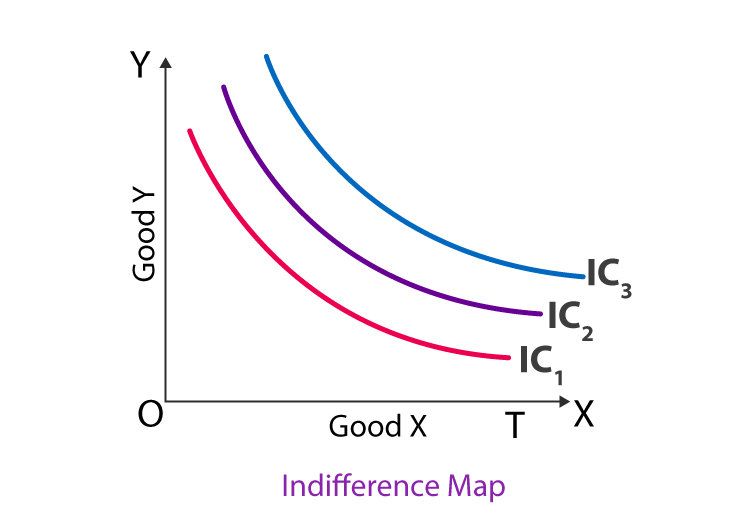
\includegraphics[width=0.7\textwidth]{images/Indifference-Map.png}

\section{Utility maximization}
\subsection{commodity and budget}
Commodity
$$L,(\mathscr{l}=1,2,...,L)$$

Commodity space
$$\mathbb{R}^{L}$$

A commodity vector is a point in commodity space
$$x=\begin{pmatrix}x_{1} \\ x_{2} \\ \vdots  \\ x_{L}\end{pmatrix}\in \mathbb{R}^{L}$$

Price vector
$$p=\begin{pmatrix}p_{1} \\ p_{2} \\ \vdots \\ p_{L}\end{pmatrix} \gg0\in \mathbb{R}^{L}$$
here much greater symbol means scarcity in market economics

Consumer's wealth level
$$w\text{ or } y$$

Affordable restraint
$$p\cdot x\leqslant w \text{ or } p\cdot x\leqslant y$$

Budget set, competitive budget restraint, Walrasian budget set, budget half-space
$$B_{p,y}=\{x\in \mathbb{R}_{+}^{L}:p\cdot x\leqslant y\} \Rightarrow B_{p,y} \text{ is convex}$$
here the restraint is caused by market

Budget hyperplane
$$\{x\in \mathbb{R}_{+}^{L}:p\cdot x= y\}$$

properties of budget set:

\begin{property}[1]
$B_{p,w} \text{ is a concave set}$
\end{property}

\begin{proof}
\begin{align}
&x,x' \in B \Rightarrow \alpha x +(1-\alpha)x' \in B
\\&x\in \mathbb{R}
\end{align}
\end{proof}

\begin{property}[2]
$B_{tp,tw} =B_{p,w}, \forall t >1$. Using $t=\frac{1}{p_{i}}$, we can set the commodity $i$ as denominations
\end{property}

\begin{proof}
\begin{align}
&B_{tp,tw}=\{x\in \mathbb{R}_{+}^{L}:tp\cdot x= tw=p\cdot x=w\}
\end{align}
\end{proof}

\begin{property}[3]
$B(p,w)\subset B(p,w'), \forall w' >w;\; B(p,w)\supset B(p',w), \forall p' >p$
\end{property}

Relationship between price and budget hyperplane
$$p \perp B_{p,y,=}$$


\subsection{UMP and deduction}

Method (i)
The tangent point of indifference curve and budget line is where one can achieve utility maximization.

Method (ii)
\begin{align}
\begin{split}
& \mathop{max}_{\{x\}} \;u(x)
\\&s.t.\; px \leqslant y
\end{split}
\end{align}

Walrasian demand correspondance
$$x(p,w)=C(B_{p,w})$$
$\Rightarrow$ singleton walrasian demand correspondance is a demand function

Marshallian demand function or Walrasian demand function
$$x=x(p,y)=\begin{pmatrix}x(p_{1},y_{1}) \\ x(p_{2},y_{2}) \\ \vdots \\ x(p_{L},y_{L})\end{pmatrix}$$

it should be

\begin{property}[homogeneous of degree zero]
meaning proportional changes in price and wealth will not effect demand
$$\forall p,w,\alpha>0:x(\alpha p, \alpha w)=\alpha^{0}x(p,w)=x(p,w)$$
and since it is defined in a Walrasian budget set, where it is homogeneous of degree zero already, the demand function must be homogeneous of degree zero as well
\end{property}

\begin{property}[Satisfying Walras' law]
\begin{align}
&\forall p \gg 0 [\forall i ,p=(p_{1},p_{2},...,p_{i},...,p_{n}),p_{i}>0],
\\&w>0 \Rightarrow p \cdot x=w, \forall x\in x(p,w)
\end{align}
\end{property}

\begin{proof}
\begin{align}
&\text{If } px<w, \exists y \in B(p,w)
\\&\text{and } y\ge x \Rightarrow py >px
\\&\Rightarrow y \succsim x
\end{align}
\end{proof}

For convience, we can use the property of being homogeneous of degree zero to set price at 1 unit for some commodities or set the wealth level at 1 unit.

Indirect utility function
\begin{align}
v(p,y)=& \mathop{max}_{\{x\}} \;u(x)
\\&s.t.\; px \leqslant y
\end{align}

Expenditure function
$$e(p,u)$$

Hicks demand function
$$x^{h}(p,u)$$

Roy's identity
$$-\frac{\frac{\partial{v(p,y)}}{\partial{p}}}{\frac{\partial{v(p,y)}}{\partial{y}}}=x(p,y)$$

Shephard's lemma
$$\frac{\partial{}e(p,u)}{\partial p}=x^{h}(p,u)$$

\section{Price change and income change}

Engel function
$$If\;p=\bar{p}\in \mathbb{R}_{+}^{n},\;x(\bar{p},w)$$

ICC, Wealth expansion path
$$E_{p}=\{x(\bar{p},w):w>0\}\in \mathbb{R}^{L}$$

Wealth effect of commodity $\mathscr{l}$ 
$$\frac{\partial x_\mathscr{l}(p,w)}{\partial w}$$

Normal good and inferior good
$$\begin{cases}&\frac{\partial x_\mathscr{l}(p,y)}{\partial y}>0 \Rightarrow \text{normal at }(p,y) \\
\\&\frac{\partial x_\mathscr{l}(p,y)}{\partial y}<0 \Rightarrow \text{inferior at }(p,y)\end{cases}$$

Total wealth effects
$$\triangledown_{w}x(p,w)= D_{w}x(p,w)=\begin{pmatrix}\frac{\partial x_{1}(p,w)}{\partial w} \\ \frac{\partial x_{2}(p,w)}{\partial w} \\ \vdots \\ \frac{\partial x_{L}(p,w)}{\partial w}\end{pmatrix}$$

Price effect on commodity $\mathscr{l}$ for price $p_{k}$ of $k$
$$\frac{\partial x_\mathscr{l}(p,w)}{\partial p_{k}}, \text{if }\mathscr{}k=\mathscr{l} \text{ then it is called self price effect}$$

Giffen good

For good $\mathscr{l}$, it is a Giffen good if 
$$\frac{\partial x_\mathscr{l}(p,w)}{\partial p_\mathscr{l}}<0$$

Complementray good

For good $\mathscr{l}$, it is a complementary good if 
$$\frac{\partial x_\mathscr{l}(p,w)}{\partial p_{j}}<0,\mathscr{l}\neq j$$

Substitute good

For good $\mathscr{l}$, it is a substitute good if 
$$\frac{\partial x_\mathscr{l}(p,w)}{\partial p_{j}}>0,\mathscr{l}\neq j$$

Total price effects
$$D_{p}x(p,w)=\begin{pmatrix}\frac{\partial x_{1}(p,w)}{\partial p_{1}}\; \dots\;\frac{\partial x_{1}(p,w)}{\partial p_{L}} \\  \ddots \\ \frac{\partial x_{L}(p,w)}{\partial p_{1}}\;\dots\;\frac{\partial x_{L}(p,w)}{\partial p_{L}}\end{pmatrix}$$

PCC, offer curve
$$x(p,\bar{w})$$


\begin{proposition}
If a $x(p,w)$ is homogeneous of degree zero, then CRTS, denoted as
\begin{align}
&\forall p,w
\\&p\cdot D_{p}x+w\cdot D_{w}x=0
\end{align}
\end{proposition}

\begin{proof}
\begin{align}
& x(tp,tw)=x(p,w),\forall \mathscr{l}=1,2,...,L
\\&\text{Take derivatives of }t \text{ on both side and moves of deduction, we have when } t=1
\\& p\cdot D_{p}x+w\cdot D_{w}x=0
\end{align}
\end{proof}

This mean proportional and simultaneous change in both price and wealth will not change demand.




Recalling that if a production function is homogeneous of degree one, it satisfies both CRTS and product exhaustion theorem.
CRTS:
$$f(\lambda x, \lambda y)=\lambda f(x,y),\lambda>1$$

Product exhaustion theorem
$$x\cdot f_{x}+y\cdot f_{y}=f(x,y)$$


\begin{proposition}[Cournot Aggregation]
If a demand function fulfils Law of Walras, then $\forall p,w \Rightarrow p_{l} D_{p_{k}}x_{l}(p,w)+x_{k}(p,w)^{T}=0$. In possible way we can imagine this as $p \times \triangle x+(\triangle p=1)\times x=0$. meaning the total expenditure is fixed, which is also called the Cournot Aggregation.
\end{proposition}

\begin{proof}
$\text{As same as to prove } p\cdot x(p,w)=w$
\end{proof}

\begin{proposition}[Engel Aggregation]
$\text{When a } x(p,w) \text{ fufils Walrasian Law}, \sum_{l=1}^{L} p_{l}\frac{\partial x_{l}(p,w)}{\partial w}=1 \text{ or } p\cdot D_{w}x(p,w)=1$, which is also called the Engel Aggregation. Meaning the change in total expenditure is equal to the change in wealth.
\end{proposition}

\section{Elasticity and aggregation}
elasticity of demand of good $i$ with respect to wealth $w$
$$\eta_{i}=\frac{\partial ln x}{\partial lnw}$$

elasticity of demand of good $i$ with respect to price $p_{i}$ of itself
$$\epsilon_{ii}=\frac{\partial ln x_{i}}{\partial lnp_{i}}$$

elasticity of demand of good $i$ with respect to price $p_{j}$ of another good $j$
$$\eta_{ij}=\frac{\partial ln x_{i}}{\partial lnp_{j}}$$

percentage of cost of good $i$ in total cost
$$S_{i}=\frac{px}{w} \Rightarrow \sum\limits_{i=1}^{n} S_{i}=1$$

Engel aggregation
$$\sum\limits_{i=1}^{n} S_{i} \eta_{i}=1$$

Cournot aggregation
$$\sum\limits_{i=1}^{n}S_{i}\epsilon_{ij}=-S_{j}$$


Substitution matrix
\begin{align}
&S(p,w)=D_{p}x(p,w)+D_{w}x(p,w) \cdot X(p,w)^{T}
\\&S_{lk}(p,w)=\frac{\partial x_{l}(p,w)}{\partial p_{k}}+\frac{\partial x_{l}(p,w)}{\partial w} x_{k}(p,w)
\end{align}




\subsection{Duality}






\section{Uncertainty}





\section{Revealed preference}
\subsection{Choice structure}

Budget line

Given price vector $p$ and income vector $y$, a budget set $B$ is defined as
$B_{p,w}=\{x|x\in \mathbb{R}_{+}^{n},px \leqslant w\}$. The border of a budget set is the budget line.

A family of budget sets $\mathscr{B}$ is denoted as
$$\{\mathscr{B}|B_{1},B_{2},...,B_{n}\}$$
$\mathscr{B}$ is a set of nonempty subset, the budget set, $B_{i}$ of the choice set $X$. It represent all possible choice sets for the choice maker, however not needed for the whole $X$.

\begin{blueblock}
\begin{note}[Family]
Since $\mathscr{B}$ is a set of sets, it is called a family.
\end{note}
\end{blueblock}


Choice rule $C(\cdot)$, or a choice function is denoted as
\begin{align}
&C:X\rightarrow X
\\& \forall B \subset \mathscr{B},C(B)\subset B
\end{align}
Notice that $C(\cdot)$ is theoretically non-empty. For every $B_{i}$ in $\mathscr{B}$, $C(\cdot)$ can always choose the best element(s). 

A choice structure is denoted as
$$(\mathscr{B},C(\cdot))$$


\begin{proposition}
$x,y \in C(\mathscr{B}) \Rightarrow x \sim y$
\end{proposition}

\begin{proof}
\begin{align}
&x,y\in C(\mathscr{B}) \Rightarrow x,y\in \mathscr{B}
\\&x\in C(\mathscr{B}) \Rightarrow x\succsim y \; (*)
\\&y\in C(\mathscr{B}) \Rightarrow y\succsim x \; (**)
\\&(*)(**) \Rightarrow x \sim y
\end{align}
\end{proof}

\subsection{Weak axiom of revealed preference}
WARP providing a reverse way to examine if the preference is rational
\begin{align}
&\exists B_{1},B_{2}\in \mathscr{B},
\\&\exists x,y \in B_{1},
\\&If\; \begin{cases}x\in C(B_{1}) \\
x,y \in B_{2}  \\
y\in C(B_{2})\end{cases}
\Rightarrow x\in C(B_{2})
\end{align}
or another version would be 
\begin{align}
&\exists B_{1},B_{2}\in \mathscr{B},
\\&\exists x,y\in B_{1}, 
\\&If\;\begin{cases}x\in C(B_{1})  \\
y\in C(B_{2})  \\
x\notin C(B_{2})
\end{cases} \Rightarrow x\notin B_{2}
\end{align}
Either way, this axiom is trying to prove that the decision maker is *self-consistent* or not paradoxy.

A revealed preference relationship $\succsim^{*}$ is denoted as
$$x\succsim^{*}y\iff\exists \{B\in \mathscr{B}|x,y\in B \;and \;x\in C(B)\}$$
Noticing that this relationship is neither of completeness nor of transitivity. Meaning $\succsim^{*}$ need not to be complete or transitive. 

\begin{blueblock}
\begin{note}
Recalling we establish the idea of completeness on $X$, not any $B$ or $\mathscr{B}$. 
\end{note}
\end{blueblock}

\begin{lemma}
$x,y\in C(B) \Rightarrow x\sim^{*} y$
\end{lemma}

\begin{lemma}
$x\in C(B),y\notin C(B) \Rightarrow x\succ^{*}y$
\end{lemma}

\begin{lemma}
$x \succsim^{*}y \Rightarrow y \neg \succ^{*}x$
\end{lemma}

some choice structure can be super wired. they may represent a rational preference yet fail to meet WARP. others may meet the WARP yet fail to represent a rational preference.

\subsection{Relationship between rational preference and revealed preference}
Now we have two ways to treat preference
$$\begin{cases}
\succsim: \text{preference relationship} \leftarrow \text{rational} \\
(\mathscr{B},C(\cdot)):\text{choice struture} \leftarrow \text{WARP}
\end{cases}$$

\subsubsection{From preference to choice}
Intuitively thinking, if someone is of ration (rational preference), he or she ought to be consistent (WARP). 

Suppose $\succsim$ is a preference relationship on $X$,
Define 
\begin{align}
&C^{*}(\cdot,\succsim):\mathscr{B} \rightarrow B
\\&\forall B \in \mathscr{B}, C^{*}(B,\succsim)=\{x\in B| \forall y \in B,x\succsim y  \}
\end{align}


\begin{redblock}
\begin{question}
what if the $B$ is an infinite set with the property of strictly increasing? can one ever search for the most preferred $x$? 
\end{question}
\end{redblock}

From now on, suppose that $\forall B \in \mathscr{B}, C^{*}(B,\succsim)\neq \varnothing$  

\begin{proposition}
Suppose $\succsim$ is rational, then the choice structure $(\mathscr{B},C^{*}(\cdot, \succsim))$ satisfies WARP.
\end{proposition}

\begin{proof}
\begin{align}
&\exists B\in \mathscr{B}
\\&x,y\in B 
\\&x\in C^{*}(B,\succsim)
\\& \Rightarrow x\succsim y \blacksquare
\\& \exists B'\in \mathscr{B}
\\&x,y\in B'
\\&y\in C^{*}(B',\succsim)
\\&y\succsim (\forall z\in B')
\\& \Rightarrow x\succsim y \succsim z \;(\text{transitivity axiom in rational preference})
\\& \Rightarrow x\in C^{*}(B',\succsim) \blacksquare
\end{align}
\end{proof}

So we can have a final conclusion about the relationship from preference relationship to choice structure: if a rational preference is captured by a choice structure, this choice structure must satisfy WARP.

\subsubsection{From choice to preference}
Now from the choice structure to preference, how does it work? If someone possesses consistency, would it be enough to assure rationality? Our guts wouldn't jump to a quick decision. Turns out, it needs some kind of restrictions to be positive.

\begin{proposition}
If choice structure $(\mathscr{B},C(\cdot))$ satisfies

(i) 
WARP

(ii) 
$\mathscr{B}$ includes all subsets of $X$ of up to three elements.

then there is one and only one rational preference can rationalize this choice structure, denoted as
$$\forall B\in \mathscr{B},C(B)=C^{*}(B,\succsim)$$
\end{proposition}

\begin{proof}
(i)
\begin{align}
\\& \text{Meaning the preference is rational: }
\\&\text{(completeness)}
\\&B:\{x,y\}\in \mathscr{B}
\\&[C(B)=x\lor y] \Rightarrow [x\succsim^{*} y] \lor [y\succsim^{*} x]\blacksquare
\\&\text{(transitivity)}
\\&\exists B:\{x,y,z\}\in \mathscr{B}, \text{ let } x \succsim^{*} y \text{ and }  y\succsim^{*} z
\\&\text{If } \; y\in C(B) \Rightarrow x \in C(B)
\\&\text{If } z\in C(B), \text{ similarly} \Rightarrow x\in C(B) 
\blacksquare
\\& \text{Thus proved}\blacksquare
\end{align}
\end{proof}

\begin{proof}
(ii)
\begin{align}
&\text{Meaning }\forall B \in \mathscr{B}, C(B)=C^{*}(B,\succsim^{*})\blacksquare
\\& \text{Let } x \in C(B),\forall y\in B,x\succsim^{*}y \Rightarrow C(B)\subset C^{*}(B,\succsim^{*})
\blacksquare
\\& \text{Let }x\in C^{*}(B,\succsim^{*}),\forall y\in B, \exists B^{y}\subset B, \text{ where } x,y\in B^{y} 
\\&\Rightarrow x\in C(B) \Rightarrow C^{*}(B,\succsim^{*})\subset C(B)\blacksquare
\end{align}
\end{proof}


\begin{proof}
(iii)

Since $\mathscr{B}$ contains all subsets of up to three elements, it assures certain binary preference relationship.
\end{proof}



Unfortunately, this restrict is arguably not strong enough in reality.

\subsection{WARP and Law of Demand}

\begin{proposition}
If a walrasian demand function $x(p,w)$ fufils WARP, for two $(p,w)$ and $(p',w')$:
If $px(p',w')\leqslant w$ and $x(p',w') \neq x(p,w$), then $p' x(p,w)>w'$.
\end{proposition}

\begin{proof}
\begin{align}
& px(p,w)=w, B(p,w) 
\\&p'x(p',w')=w', B(p',w')
\\&\text{If } px(p',w')\le w \Rightarrow x(p',w')=x'\in B(p,w)
\\&\text{If }x\notin B(p',w') \Rightarrow p' x(p,w)>w'
\end{align}
\end{proof}

Or we can prove it using WARP.
\begin{proof}
\begin{align}
&\begin{cases}
px(p,w)=w \\
p'x(p',w')=w' \\
px(p',w')\leq w\end{cases} \Rightarrow p'x(p,w)>w
\end{align}
\end{proof}

Slutsky wealth compensation
$$w=px(p,w)\Rightarrow \triangle w=w'-w=\triangle p \cdot x(p,w)$$

WARP and Slutsky wealth compensation
\begin{align}
& x(p,w) \text{ fulfils Walrasian Law, it fulfils also the WARP }\iff
\\&(p,w)\rightarrow(p',w')=(p',w'=p'x(p,w)): (p'-p)[x'(p,w')-x(p,w)]\leqslant0
\end{align}


\section{Classic Demand Theory}
\subsection{Preference relationship}
\textbf{A. desired assumption: the more goods, the better}

monotonicity
\begin{align}
&\text{If }x\in X \text{ and } y \gg x \text{ meaning }y>x \Rightarrow \succsim \text{is weak monotonic}
\end{align}

local non-saturation assumption:
\begin{align}
&\text{If }\exists \succsim \text{ on } X, \forall x\in X \text{ and } \forall \epsilon>0, \text{ always } \exists y \in X \text{ that}
\\&||y-x||\le \epsilon \text{ and }y>x
\\&\Rightarrow \text{the preference relationship }\succsim \text{ is local non-satisfying.}
\end{align}

this is an assumption weaker than monotonicity assumption (the order in term of weak and strong is strictly monotonic $>$ weak monotonic $>$ local non-saturation)

Based on $x$ and $\succsim$, three related sets are defined:

Indifference set
$$\{y\in R: y \sim x\}$$
(local non-saturation ensures the existence of indifference curves in two-dimensional space)

Upper contour set
$$\{y\in R: y \succsim x\}$$

Lower contour set
$$\{y\in R: x \succsim y\}$$

\textbf{B. Convexity assumption: }

diversity, diminishing marginal utility, diminishing marginal rate of substitution
$\succsim$ on $X$ is convex if
$$\forall x \in X, \text{ the upper contour set }\{y\in R: y \succsim x\} \text{ is convex} $$
That is,
$$
\text{If }y\succsim x, \forall \alpha \in [0,1],\alpha y+(1-\alpha)z \succsim x
$$
A real commodity set may not satisfy the convexity assumption, but for the convenience of analysis, we need to assume convexity

\textbf{C. Other preference relations}

Similar preferences
$\succsim$ is similar if all indifference sets can be extended in equal proportion along any ray and connected together. That is, if $x \sim y$, then $ax \sim ay, \forall a \ge 0$.

Quasi-linear preference (omitted)

\subsection{Utility}
\textbf{A. Lexicographic preference relation}
$$X=\mathbb{R}^{2}_{+},x\succsim y:\text{either [}x_{1} > y_{1} \text{], or [} x_{1}=y_{1} \text{ and } x_{2} \ge y_{2}\text{]}.$$
This is rational, monotonic, and convex, but does not satisfy the continuity assumption, and there is no utility function

\textbf{B. Continuity assumption of preference}
If the preference relation of X is continuous, then the previous preference relation can still be retained in the limit operation

If it is continuous, then the upper and lower contour sets are closed sets
If it is continuous, then there is a utility function $u$ that can represent the continuous relation
If $\succsim$ is convex, then there is a $u$ that can represent $\succsim$, then $u$ is quasi-concave

\subsection{Utility maximization problem}
Assume that consumers have rational, continuous, and locally unsaturated preference relations, and use continuous functions $u(\cdot)$ to represent these preferences

\begin{redblock}
\begin{question}
What is the demand function of the CD function $u=k x_{1}^{\alpha} x_{2}^{1-\alpha},\alpha \in (0,1),k>0$?
\end{question}
\begin{align}
&\mathop{max}\limits_{x}\; u(x)
\\&s.t. \; px=w
\\&\text{Make some changes so that }\ln u=\ln k +\alpha \ln x_{1} +(1-\alpha)\ln x_{2}
\\&FOC: \nabla u(x)=\lambda p
\\& \Rightarrow x_{1}=\frac{\alpha w}{p_{1}},x_{2}=\frac{(1-\alpha)w}{p_{2}}
\end{align}
\end{redblock}



\begin{redblock}
\begin{question}
find the demand function based on $\mathop{max}\limits_{x}\;u(x)=[\sum\limits_{i=1}^{n} x_{i}^{\frac{\alpha-1}{\alpha}}]^{\frac{\alpha}{\alpha-1}}\;s.t.\; \sum\limits_{i=1}^{n} p_{i}x_{i}=w$
\end{question}
\begin{align}
&FOC: \frac{\alpha}{\alpha-1}[\sum\limits_{i=1}^{n} x_{i}^{\frac{\alpha-1}{\alpha}}]^{\frac{\alpha}{\alpha-1}-1}\frac{\alpha-1}{\alpha}x_{j}^{\frac{\alpha}{\alpha-1}-1}=\lambda p_{j},\forall j =1,2,...,n
\\&\text{Multiply both sides with }x_{j}
\\&\frac{\alpha}{\alpha-1}[\sum\limits_{i=1}^{n} x_{i}^{\frac{\alpha-1}{\alpha}}]^{\frac{\alpha}{\alpha-1}-1}\frac{\alpha-1}{\alpha}x_{j}^{\frac{\alpha}{\alpha-1}}=\lambda p_{j}x_{j},\forall j =1,2,...,n
\\&\text{Start from j=1 and add up to n}
\\&[\sum\limits_{i=1}^{n}x_{i}^{\frac{\alpha-1}{\alpha}}]^{\frac{\alpha}{\alpha-1}}=\sum\limits_{j=1}^{n}\lambda p_{j}x_{j}=\lambda w
\\&x_{j}^{-\frac{1}{\alpha}}=p_{j}[\sum\limits_{i=1}^{n}x_{i}^{\frac{}{}}]
\end{align}
\end{redblock}


First-order conditions for corner solutions: 
\begin{align}
&x_{l}^{*}=0, \frac{\partial u_{l}(x^{*})}{\partial x_{l}}\le \lambda p_{l}
\\&x_{l}^{*}>0, \frac{\partial u_{l}(x^{*})}{\partial x_{l}}= \lambda p_{l}
\end{align}


\textbf{Indirect utility function} $v(p,y)$:
\begin{property}[HD0]
\begin{align}
&v(p,w)=v(tp,tw),\forall t >0
\\&B_{p,w}=B_{tp,tw}
\\&\Rightarrow x(p,w)=x(tp,tw)
\\&\Rightarrow v(p,w)=u(x(p,w))=u(x(tp,tw))=v(tp,tw)
\end{align}
\end{property}

\begin{property}
Non-increasing for $p$, strictly increasing for $w$
\end{property}

\begin{proof}
$$(p1,p2)\rightarrow (p1',p2)\Rightarrow B_{p,w}\subseteq B_{p',w} \Rightarrow v(p',w)\ge v(p,w)$$
\end{proof}

\begin{property}[quasi-convex]
That is, the set $\{(p,w):v(p,w)\le D\}$ is convex for any $D$
\end{property}

\begin{proof}
\begin{align}
&\text{Assume that }(p1,w1),(p2,w2),
\\&v(p1,w1)\subseteq D,v(p2,w2)\subseteq D
\\&(p3,w3)=\alpha(p1,w1)+(1-\alpha)(p2,w2)=[\alpha p1+(1-\alpha)p2,aw1+(1-\alpha)w2],\forall \alpha>0
\\&
\end{align}
\end{proof}

\begin{property}[Minimize expenditure EMP]
\end{property}


\begin{proof}
Let $p\gg 0$ and $u>u(0)$, $u(\cdot)$ continuous
\begin{align}
\begin{split}
&\mathop{min}\limits_{x\ge0}\; px
\\&s.t. u(x)\ge u
\end{split}
\\&\Rightarrow  x^{h}(p,w)
\\&e(x^{h}(p,u))=e(p,w)
\end{align}
\end{proof}


\subsection{Duality}
EMP is the dual problem of UMP

\begin{proposition}[a]
$x^{*}$ is the optimal consumption bundle of UMP. For a given target utility $u(x^{*})$, $x^{*}$ is also the most optimal in EMP, and the minimum expenditure is exactly $w$. $x^{h}(p,u)=x(p,e(p,u))$
\end{proposition}

\begin{proposition}[b]
$x^{*}$ is also the most optimal in EMP. When the wealth level is $p x^{*}$, $x^{*}$ is also the best in UMP, and the maximum utility is $u$. $x(p,w)=h(p,u(p,w))$
\end{proposition}

\begin{proof}[a)]
\begin{align}
& x^{*}\in x(p,w) \iff \begin{cases}
px^{*}=w \\
u(x^{*})\ge u(x'), \forall x'p \le w\end{cases}
\\&\text{If } x^{*}\notin x^{h}(p,u)
\\\begin{split}
&\min\limits_{x} px
\\&s.t. u(x)\ge u(x^{*})
\end{split}
\\&\exists \bar{x}, p\bar{x}<p x^{*}, u(\bar{x})\ge u(x)
\\&u(\bar{x}) \ge u(x^{*})\ge u(x'),\forall x'p\le w
\\&u(\bar{x})\ge u(x'),\forall x'p\le w
\\&\Rightarrow \bar{x} \text{ is the optimal option in UMP},\bar{x} \in x(p,w)
\\& \Rightarrow x^{*} \in x^{h}(p,u)
\end{align}
\end{proof}

\begin{proof}[b)]
\begin{align}
& \text{Assume that }x^{*} \notin x(p,w)
\\&\exists \bar{x},p\bar{x}\le w, u(\bar{x})>u(x^{*}),px'<w
\\&u(x')\ge u(x^{*}),px'<w=px^{*}
\\&x'=t\bar{x}, t\in (0,1)
\\&u(x')\ge u(x^{*}), px'<w
\\&u(x')\ge u(x^{*}),px'<w=px^{*}
\\&x^{*} \notin x^{h}(p,u) \text{ and } x^{*} \text{ is the optimal option are paradox}
\\&\Rightarrow x^{*} \in x(p,w)
\end{align}
\end{proof}

\textbf{Expenditure function} $e(p,u)$ 

\begin{property}[HD1 with respect to P]
\begin{align}
&e(p,u)=px_{1},\forall x \in x^{h}(p,u)
\\&e(tp,u)=tpx_{2},\forall x_{2}\in x^{h}(tp,u)
\\&e(tp,u)=t e(p,u)
\\&tpx_{1}=tpx_{2} \Rightarrow x_{1}=x_{2}
\\&x^{h}(p,u)=x^{h}(tp,u) \Rightarrow \text{HD}0
\end{align}
\end{property}


\begin{property}Regarding u is strictly increasing and p is non-decreasing
\end{property}

\begin{proof}
\begin{align}
&u_{1} > u_{2} \Rightarrow e(p,u_{1})>e(p,u_{2})
\\&\text{Assume that }u_{1}>u_{2},e(p,u_{1})\le e(p,u_{2}) \text{ holds true}
\end{align}
\end{proof}

\begin{property}Regarding the concave function of $p$
\end{property}

\begin{proof}
\begin{align}
&e[\alpha p_{1}+(1-\alpha)p_{2},u]\geqslant \alpha e(p_{1},u)+(1-\alpha)e(p_{2},u)
\\&e[\alpha p_{1}+(1-\alpha)p_{2},u]=[\alpha p_{1}+(1-\alpha)p_{2}]x_{3}
\\&x_{3} \in x^{h}(\alpha p_{1}+(1-\alpha)p_{2},u)=\alpha p_{1}x_{3}+(1-\alpha)p_{2}x_{3}
\\&\ge a p_{1}x_{1}+(1-\alpha)p_{2}x_{2}=\alpha e(p_{1},u)+(1-\alpha) e(p_{2},u)
\end{align}
\end{proof}


\textbf{Hicks demand function}

Properties of Hicks demand function
\begin{property}[HD0]
\end{property}

\begin{property}[No excess utility]
$x\in x^{h}(p,u),u(x)=u$
\end{property}


\begin{property}
Hicks demand functino is the derivative of $e(p,u)$ with respect to $p$
\end{property}

\begin{proposition}[Hicks demand satisfies the law of compensation of demand]
For the price change of Hicks wealth compensation, the movement direction of demand and price is opposite
$$(p'-p)[x^{h}(p',u)-x^{h}(p,u)]\leqslant 0$$
\end{proposition}

\begin{proof}
\begin{align}
&x^{h}(p',u) \text{ is the optimal choice at price }p'
\\&\Rightarrow p'x^{h}(p',u)\le p' x^{h}(p,u)\;(*)
\\&\text{Same for at the price }p,
\\&\Rightarrow px^{h}(p,u)\le p x^{h}(p',u)\;(**)
\\&p' x^{h}(p',u)+p x^{h}(p,u)\le p' x^{h}(p,u)+p x^{h}(p',u)
\\&(p'-p)(x^{h}(p',u)-x^{h}(p,u))\le 0
\end{align}
\end{proof}

Slutsky equation
$$\frac{\partial x^{h}(p,u)}{\partial p_{k}}=\frac{\partial x_{l}(p,w)}{\partial p_{k}}+\frac{\partial x_{l}}{\partial w}x_{k}(p,w)$$

\section{Choice under uncertainty}
Outcome
$$X=(x_{1},x_{2},...,x_{n})$$

lottery
\begin{align}
&\text{A set of possibilities }l=(P_{1},P_{2},...,P_{n}),\forall P_{i}\ge 0, \sum\limits_{i=1} Pi=1
\\&\Rightarrow L=(P_{i}x_{i})
\end{align}

compound lottery
\begin{align}
&\exists \text{an amount of }k \text{ lotteries } L_{k}=(p_{i}^k)
\end{align}
Complex lotteries can be simplified to simple lotteries
If two different complex lotteries have the same lottery after simplification, then we consider them to be the same

Simplex
Geometric figure used to represent lotteries (simple or complex)
$$\triangle=\{P\in \mathbb{R}_{+}^{n}:P_{1}+...+P_{n}=1 \}$$

Alternative set
$\mathscr{L}$

Assumption: $\succsim$ is complete and transitive
Complete means $\forall L,L'\in \mathscr{L}$, which satisfies $L\succsim L'$ or $L'\succsim L$ or both
Transitive means $\forall L,L',L''\in \mathscr{L},L\succsim L',L'\succsim L''$, then $L\succsim L''$

Continuity axiom (assumption)
$\succsim$ is continuous on $\mathscr{L}$ if for $\forall L,L',L''\in \mathscr{L}$, the set $\{\alpha\in [0,1]:\alpha L+(1-\alpha) L' \succsim L''\}\subset [0,1]$ and the set $\{\alpha\in [0,1]:L''\succsim \alpha L+(1-\alpha) L' \}\subset [0,1]$ are both continuous

Independence axiom (assumption)
\begin{align}
&\forall L,L',l'' \in \mathscr{L}, \exists \alpha \in [0,1],
\alpha L+(1-\alpha )L''\succsim \alpha L' +(1-\alpha)L'' \iff L \succsim L'
\end{align}

Conclusion:
a): $L\succ L'$ if and only if $\alpha L+(1-\alpha)L''\succ \alpha L' +(1-\alpha)L''$
b): $L\sim L'$ if and only if $\alpha L+(1-\alpha )L'' \sim L' +(1-\alpha)L''$

Expected utility function
$U:\mathscr{L}\rightarrow \mathbb{R}$
$U(L)=\sum\limits_{i} P_{i}u_{i}$

Conclusion:
a) VM utility function $\iff$ linear
b) $\succsim \Rightarrow U(L), V(L)=\alpha U(L)+\beta,\alpha >0$ in $\mathscr{L}$

Existence theorem (expected utility theorem)
Preferences in lottery space are complete, transitive, continuous, and independent, so preferences can be expressed by expected utility functions.

\newpage
\part{FIRM AND SUPPLY THEORY}


\newpage
\section{Firm}
production possiblity set
$$\mathbb{R}^{L}$$

production vector
$$y=(y_{1}, y_{2},...,y_{L})\in \mathbb{R}^{L}$$

production process
$$y^{A} \rightarrow y^{B} \Rightarrow y=y^{A}-y^{B}=y^{output}-y^{input}$$

production feasibility set
$$Y=\{y\in \mathbb{R}^{L}|y \text{ if feasible allowed by current technology}\}$$

transformation function
\begin{align}
&T: \mathbb{R}^{L} \rightarrow \mathbb{R}
\\&\iff
\\&\text{(1). } \forall y \in Y, T(y) \leqslant 0
\\&\text{(2). }T(y)<0,\text{ if } \exists y'\in Y,y'>y
\\&\text{(3). }T(y)=0, \neg \exists y \in Y, y' >y
\end{align}
transfer function can be consider a sort of measurement of efficiency of production, where the hyperplane is set of the most efficient vectos.

input requirement set
\begin{align}
&\text{Let } q \geqslant 0\in \mathbb{R}^{m}, x \geqslant 0 \in \mathbb{R}^{L-m},y=(q,-x) \Rightarrow V(q)=\{x\in \mathbb{R}^{L}|(q,-x)\in Y\}
\end{align}
if $q^{1}\geqslant q^{2}$, then $V(q^{1}) \subset V(q^{2})$

Production function
\begin{align}
&\text{Define }m=1,L-m=L-1
\\&f:\mathbb{R}^{L-1} \rightarrow \mathbb{R} \text{ is a production function if } (f(x),-x)\in Y \text{ and } T(f(x),-x)=0
\end{align}

CD production function
$$f(x)=A \sum\limits_{i=1}^{L-1}x_{i}^{a_{i}}$$

Leontief production function
$$f(x)=min\{a_{1} x_{1},...,a_{n}x_{n}\}$$

linear production function
$$f(x)=\sum\limits_{i=1}^{L-1}a_{i}x_{i}$$

two production factors
$$\text{CD: }f(x)=ax_{i}^{\alpha}x_{2}^{1-\alpha},\text{Leontif: }f(x)=min\{a_{1}x_{1},a_{2}x_{2}\}$$

a special case with two production factors
$$f(x_{1},x_{2})=[ax_{1}^{\rho}+bx_{2}^{\rho}]^{\frac{1}{\rho }},a+b=1 \Rightarrow \begin{cases} \rho \rightarrow 0, \text{ CD}\\
\rho=1, \text{ linear} \\
\rho \rightarrow -\infty ,\text{ Leontief}
\end{cases}$$

```ad-abstract
title: Quiz of CES to Leontief


```


properties of production set
(i)
closed, meaning the hyperplane is attained
(ii)
irreversable 
$$\text{if } y\in Y, \text{then }-y\notin Y$$
(iii)
$$\{0\}\subset Y$$
(iv)
no free lunch
$$y\in Y,y \geqslant 0 \Rightarrow y=0$$

(v)
disposal at freedom
$$\text{If } y \in Y, y' \leqslant y \Rightarrow y' \in Y$$

(vi)
additivity
$$\forall y,y' \in Y,\;y+y'\in Y$$
(vii)
convexity
$$\forall x,y \in Y,\exists \alpha\in [0,1],\alpha x+(1-\alpha)y\in Y$$

Marginal product
\begin{align}
q=f(k,l) \Rightarrow \frac{\partial q}{\partial k}=f_{l} \text{ or } \frac{\partial q}{\partial l}=f_{k}
\end{align}

diminishing marginal product
$$\frac{\partial ^{2}f}{\partial k^{2}} <0\text{ or } \frac{\partial ^{2}f}{\partial l^{2}}<0 \text{, but } \frac{\partial ^{2}f}{\partial l \partial k} \text{ can be positive.}$$

marginal rate of substitution
$$
\exists f(k,l), MRST=\frac{dk}{dl}=|\frac{MP_{l}}{MP_{k}}|=-\frac{MP_{l}}{MP_{k}}
$$

elasticity of substitution
$$
\delta=\frac{d\ln \frac{k}{l}}{d\ln |MRST|}
$$
\begin{redblock}
\begin{question}[Quiz of calculating elasticity of CES function]
\begin{align}
&q=f(k,l)=(k^{\rho}+l^{\rho})^{\frac{\gamma}{\rho}}
\\&\Rightarrow MRST=-\frac{f_{l}}{f_{k}}=-(\frac{k}{l})^{1-\rho}
\\&\Rightarrow \delta=\frac{dln \frac{k}{l}}{dln |MRST|}=\frac{1}{1-\rho}
\end{align}
\end{question}
\end{redblock}

\section{PMP}
profit maximization problem, PMP
\begin{align}
&\text{For a production function }f(x)=f(x_{1},x_{2},...,x_{n})
\\& \text{The gradient is }\nabla f(x)=[\frac{\partial f}{\partial x_{1}},\frac{\partial f}{\partial x_{2}},...,\frac{\partial f}{\partial x_{n}}]
\\&\text{Given production feasibility set } Y \text{ and price vector } P\gg 0
\\&\text{The profit maximization is denoted as}
\\&\begin{cases}
& \mathop{max}\limits_{y} \;py
\\& s.t. \; T(y) \leqslant 0  \\
\end{cases}
\text{ or } 
\begin{cases}
& \mathop{max}\limits_{y} \;py
\\&s.t. \;y\in Y  \\
\end{cases}
\\&\Rightarrow \pi(P)=max \{py:y\in Y\}
\\&y_{\text{product provided}}=\{y\in Y,py=\pi(p) \}
\\&
\\&\text{If transformation function T(y) is differentiable, then} 
\\&
\text{the solution to PMP can also be denoted as}
\\&
\begin{cases}\text{FOC: }p=h \nabla T(y^{*}) \Rightarrow \frac{\partial f}{\partial x}=\frac{w_{x}}{p}
\\\text{SOC: } D^{2}T(y^{*}) \text{ is negative half finite}
\end{cases}
\end{align}

properties of profit function
\begin{property}
Homogeneous with degree of $1$ with respect to price vector $p$
\end{property}

\begin{proof}
\begin{align}
\\& \pi(tp)=tp \cdot y^{*}= \pi(p)=t \cdot py^{*}
\\&\iff 
\begin{cases}
&\text{(1)  } \forall y \in Y(tp) \Rightarrow y \in Y(p)
\\&\text{(2) }\forall y \in Y(p) \Rightarrow y \in Y(tp)
\end{cases}
\end{align}
\end{proof}

\begin{proof}
\begin{align}
&\text{(1):}
\\& \forall y \in Y(p), py \geqslant py',\forall y' \in Y(p)
\\&(tP)y\geqslant (tP)y',\forall y' \in Y
\\&y\in Y(P_{1}=tp)
\\&
\\&\text{(2):}
\\&\forall y \in Y(tp), tpy \geqslant tpy',\forall y' \in Y(p)
\\&(tp)y\geqslant (tp)y',\forall y' \in Y
\\&y\in Y(P_{2}=tp)
\end{align}
\end{proof}

2.
profit function is a concave function
$$\pi[ap_{1}+(1-a)p_{2}]\leqslant a\pi(p_{1})+(1-a)\pi(p_{2})$$

```ad-question
title: Proving

\begin{align}
&\pi(p1)=p1y1\ge p1y3
\\&\pi(p2)=p2y2 \ge p2y3
\\&a \pi(p1)+(1-a)\pi(p2)\ge ap1y3+(1-a)p2y3=[ap1+(1-a)p2]y3=\pi(ap1+(1-a)p2)
\end{align}
```

3.
Shephard's lemma
$$\frac{\partial \pi(p)}{\partial p }=y(p)$$

```ad-question
title: Proving
\begin{align}
&\pi(p)=\mathop{max}\limits_{y} py \; s.t. T(y)\leqslant 0
\\&L(p,\phi)=py-\phi T(y)
\\&\frac{\partial L}{\partial p}=y-\phi \frac{\partial T}{\partial p}=0
\end{align}

```

$$$$

4.
law of supply
```ad-question
title: Proving

\begin{align}
&\pi(p_{s})=y_{s},\pi(p_{t})=y_{t}
\\&\Rightarrow p_{s}y_{s}\ge p_{s}y_{t},p_{t}y_{t}\ge p_{t}y_{s}
\\& \Rightarrow p_{s}y_{s}+p_{t}y_{t}\ge p_{s}y_{t}+p_{t}y_{s}
\\&\Rightarrow (p_{s}-p_{t})(y_{s}-y_{t})\ge 0
\end{align}
```

\section{CMP}
cost minimization
From production plan $y=(q,-x)$, we see two simultaneous decisions in a single move.
in the case $y=(y_{1})$

goods
$$q$$

factors
$$x$$

factor price
$$w$$

conditional factor demand function
\begin{align}
x(q,w)=\;&\mathop{min}\limits_{x}\; wx
\\&s.t.\;f(x)\geqslant q
\end{align}

cost function
$$C(w,q)=x(q,w)\cdot w$$

minimization of cost function
\begin{align}
& \text{For a cost function } C(w,q)=x(q,w)\cdot w,
\\& FOC: \; w=h \nabla f(x^{*}), \exists h\ge 0
\\&SOC: \; D^{2}f(x^{*}) \text{ is negative half-finite}
\end{align}

```ad-info
title: Case

\begin{align}
&\mathop{min}\limits_{l,k} \;c=wl+rk
\\&s.t. f(l,k)\ge q
\\&\Rightarrow \text{Using Lagrange's multiplier }L(l,k,\phi)=wl+rk-\phi[f(k,l)-q]
\\& \text{Equilibrium: } \begin{cases}
w=\phi f'_{l} \\
r=\phi f'_{k}\end{cases}
\end{align}
```

properties of cost function
\begin{align}
&c(w,q)=w\cdot x^{*},x^{*}\in x(w,q)
\end{align}
1.
noncreasing of $q$ and $w$

```ad-question
title: Proving

\begin{align}
&\text{As proving }q1\ge q2 \Rightarrow c(w,q1)\ge c(w,q2)
\\&c(w,q1)=wx1,x1\in x(w,q1),x1 \in V(q1)
\\&\text{If }q1\ge q2, V(q1)\subset V(q2)
\\&c(w,q2)=wx2\le wx1,x2\in x(w,q2),x2 \in V(q2)
\end{align}
```

2.
homogeneous with degree of $1$ with respect to $w$

```ad-question
title: Proving

\begin{align}
&c(aw,q)=aw\cdot x^{*},x^{*} \in x(aw,q)
\\&a\cdot c(w,q)=a\cdot w x^{**},x^{**}  \in x(w,q)
\\&\Rightarrow \text{As proving}\begin{cases}
\forall x\in x(w,q) \Rightarrow x\in x(aw,q) \\\forall x\in x(aw,q) \Rightarrow x\in x(w,q) 
\end{cases}
\\& \forall x \in x(w,q),awx\le awx', \forall x' \in V(q)
\\& \forall x \in x(aw,q), wx\le wx', \forall x' \in V(q)
\end{align}
```

3.
cost function is a convex function with respect to $w$
$$C[aw1+(1-a)w2]\ge a C(w1)+(1-a)C(w2), \forall a \in [0,1]$$
the convexity of cost function is to assure the slower than change of price cost thus the availablity to properly achieve optimization.

```ad-question
title: Proving

\begin{align}
& C[aw1+(1-a)w2]\ge a C(w1)+(1-a)C(w2), \forall a \in [0,1]
\\& C(w1)=w1x1\le w1x3
\\&C(w2)=w2x2\le w2x3
\\&aC(w1)+(1-a)C(w2)\le aw1x3+(1-a)w2x3=C(aw1+(1-a)w2)
\end{align}
```


\newpage
\part{GAME THEORY}

\newpage
\section{Game theory}
Complete information stastic game theory: Nash Equilibrium
Incomplete information stastic game theory: Subgame Perfection Nash Equilibrium

\subsection{CISG: NE}
Participants
$$I=\{1,2,...,n\}$$

Strategy
\begin{align}
&S_{i}=\{s_{1},s_{2},...,s_{n}\} \text{ for the particular participant } i,\text{ whereas }S \text{ for all participants}
\\&s=\{s_{ij}\},\text{ where } i \text{ stands for participant and }j \text{ stands for each action}
\end{align}

Payoff structure
$$\pi(s_{ij})$$

Information
$$\text{As literally.} \begin{cases}\text{Complete information} \\
\text{Incomplete information}
\end{cases}$$

Strictly inferior strategy
\begin{align}
&s_{i}, s_{i}' \text{ are two strategies of the participant }i,
\\&\forall s_{-i}\in S_{-i}, \pi(s_{i}',s_{-i})>\pi(s_{i},s_{-i})
\\&\Rightarrow s_{i}' \text{ is strictly superior to }s_{i} \text{ and }s_{i} \text{ is strictly inferior to }s_{i}'
\end{align}
By the repetition of elimination of strictly inferior strategies, we will have the according Nash equilibrium.

Nash Equilibrium
\begin{align}
&\text{The strategic combination }s^{*}=(s_{1}^{*},s_{2}^{*},...,s_{n}^{*}) \text{ is a Nash Equilibrium if and only if}
\\& \forall s_{i}\in S_{i},
\\&\pi_{i}(s^{*})\geqslant \pi_{i}(s_{i},s_{-i}^{*}),i=1,2...,n
\\&(s_{i},s_{-i}^{*})=(s_{1}^{*},s_{2}^{*},...,s_{n}^{*}) 
\end{align}

Mixed strategy Nash equilibrium
pure strategy is a special case of mixed
\begin{align}
&\text{A strategic combination }p^{*}=(p_{1}^{*},p_{2}^{*},...,p_{n}^{*}) \text{ is a MSNE if and only if}
\\&\forall p_{i}\in P_{i},\pi_{i}(p^{*})\geqslant \pi(p_{i},P_{-i}^**),i=1,2...,n
\\&\text{where } (p_{i},p_{-i}^{*})=(p_{1}^{*},p_{2}^{*},...,p_{n}^{*})
\end{align}






\end{document}